\documentclass[a4paper]{article}

\usepackage{amsmath}
\usepackage{algorithm}
\usepackage{algorithmic}
\usepackage{hyperref}
\usepackage{graphicx}
\usepackage[left=3cm, right=3cm, bottom=3cm, top=3cm]{geometry} 
\graphicspath{ {./images/} }

%opening
\title{Image Mosaicking \\ Study Week Fascinating Informatics}
\author{Adrian W\"alchli \\ Computer Vision Group \\ University of Bern}

\begin{document}

\maketitle
\tableofcontents
\newpage


\section{Introduction}
	\subsection{Welcome to the Institute of Computer Science}
		The Institute of Computer Science, Prof.\@ Paolo Favaro and I welcome all participants of the study week ``Fascinating Informatics''.
		As every year, we prepare a unique student project that promotes computer science with a glimpse into the research at the University of Bern.
		Our institute consists of five research groups: Computer Vision Group (CVG), Communications and Distributed Systems (CDS), Logic and Theory Group (LTG), Software Composition Group (SCG) and Computer Graphics Group (CGG).
		I am a first-year PhD student from the Computer Vision Group supervised by Prof.\@ Paolo Favaro. 
		I will be the tutor for your group project and it is my job to guide you and answer any questions you have or help with problems.
		I am very much looking forward getting to know you and work with you.
		It is the first time I design a project like this for the study week, so I am curious to hear your feedback!
		
	
	\subsection{Image Mosaicking}
		\begin{figure}
			\centering
			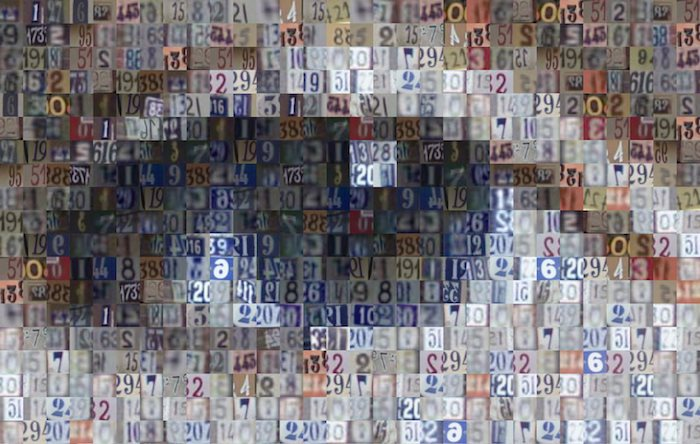
\includegraphics[width=0.7\linewidth]{eye-mosaic}
			\caption{Example mosaic using house numbers.}
			\label{fig:eye-mosaic}
			\label{fig:mosaicking-example}
		\end{figure}
		In this project, you will develop an algorithm that intelligently selects and arranges small image patches to form a mosaic of a given target image.
		An example of this is shown in figure~\ref{fig:mosaicking-example}. 
		The target image in this example is the lion, and the image patches are a random collection of images from the internet down-scaled to a smaller resolution.
		In terms of content, these small patches have nothing in common with the target image.
		In order to create a mosaic of an image, one has to define a similarity measure to be able to compare an arbitrary image patch with a region in the target image. 
		Although humans are very good at judging images by their content and appearance, you can imagine that it would still take a lot of time for a human to manually assemble a mosaic like the one shown in figure~\ref{fig:mosaicking-example}.
		In this project, you will learn how a computer can ``learn'' to compare image patches and automatically create a mosaic for any image.
	
	\subsection{Prerequisites}
		You will use Python as a programming language. 
		It is of course beneficial to have little experience with Python, or any other language, but it is not a requirement.
		Since Python is very beginner friendly, you will be able to pick it up very fast. 
		And you will like it!
		And in any case, your tutor will help you to get prepared for the programming.
		
		We will provide a computer for each student, but it is good to have your personal notebook with you for researching, taking notes etc.
	
	\subsection{Learning Outcome}
		After successful completion of this one-week project, you will  %acquired the following knowledge and skills.
		\begin{itemize}
			\item have a basic understanding of Machine Learning and Computer Vision,
			\item know how to implement and/or apply algorithms in Machine Learning and Computer Vision,
			\item have acquired skills for scientific Python programming,
			\item know how to write a scientific report and create a poster summarizing your research and results,
			\item get a better picture of what academic research looks like,
		\end{itemize}
		and hopefully be proud of your work!
	

\section{Preparation}
	Before starting with the project, you should read this document completely to get an overview of what the contents are and what we expect from you.
	We provide three Linux computers with all necessary tools installed and accessible in the desktop menu. 
	\\ \\
	\textbf{Username:} studi\\
	\textbf{Password:} rubberband
	\\ \\
	The code you have to work with is already set up.
	It is located inside the \emph{Documents} folder in your home directory. 
	Try to understand the file- and folder structure, then quickly go through all assignment files and study the comments (lines that start with \#).

	
\section{Theory}

	\subsection{Understanding the Computer Vision Problem}
		In the context of computer science, an image is simply an array of numbers where each number represents the intensity of light shown in one pixel.
		Such an image is usually taken with a digital camera that -- for a short period of time -- exposes its sensor to the light passing through the aperture.
		Depending on the camera, a small amount of low-level processing (brightness adjustments, sharpening, white balance, etc.\@) is applied to the pixel values read from the sensor.
		However, this type of processing does not require any knowledge of the contents in the image.
		What if we want to do more? 
		Here are some examples of Computer Vision problems that are too complex to solve just by ``looking'' at the raw pixel data:
		\begin{itemize}
			\item Detecting a face in an image 
			\item Solving a jigsaw puzzle
			\item Generating a caption for an image
			\item Removing the background in an image (semantic segmentation)
			\item Identifying and classifying a tumor in an x-ray image
		\end{itemize}
		There are many more examples of problems like these that are not that hard for a human to solve, but humans are slow and cannot do it reliably sometimes.
		
	\subsection{Image Mosaicking}
		The problem of Image Mosaicking can be described as follows.
		We are given a large dataset of small image patches (say $32 \times 32$ pixels) and an arbitrary user-supplied target image (say $1024 \times 1024$ pixels).
		The Mosaicking algorithm must select patches from the dataset and arrange them in a grid to form an output image of the same size as the target image, depicting the same object or scene.
		Figure~\ref{fig:mosaicking-working-and-not-working} shows an example of a failing algorithm that randomly chooses image patches, and a working algorithm that produces the desired result.
		\begin{figure}
			\centering
			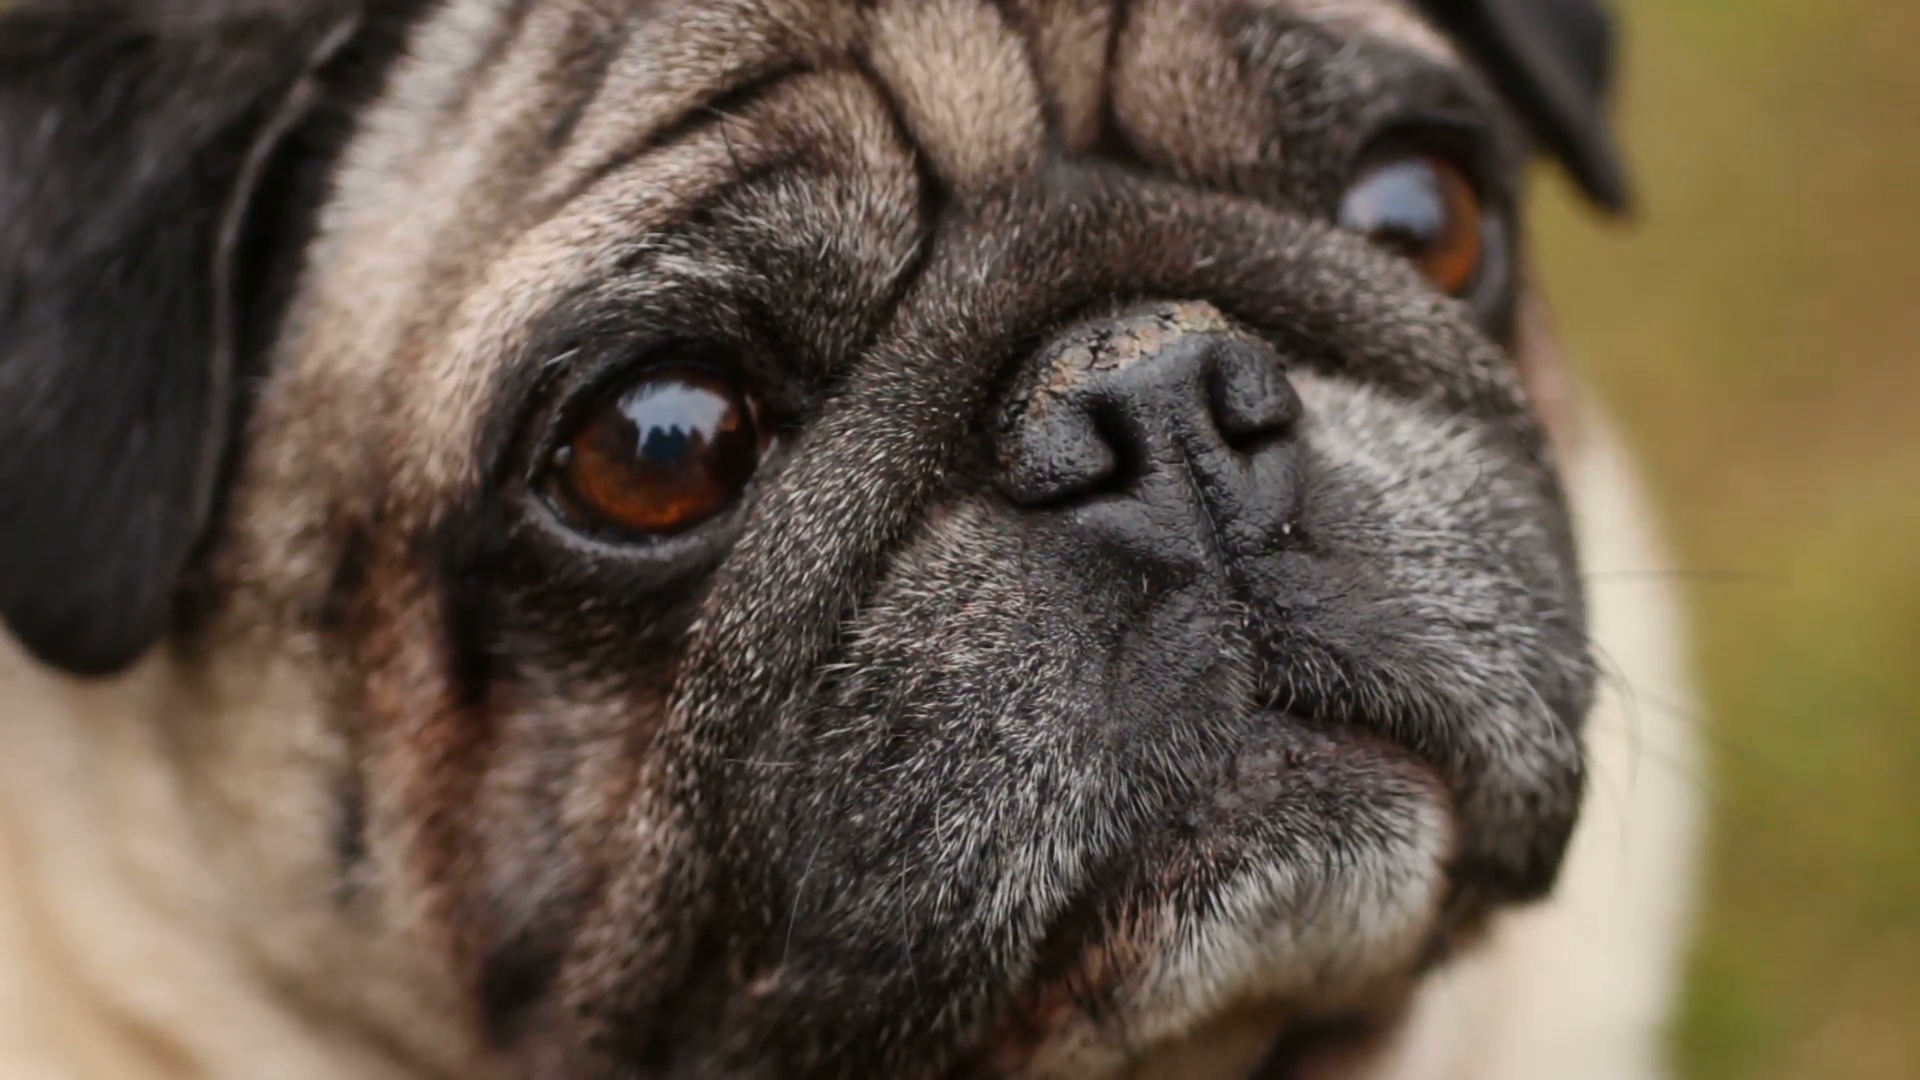
\includegraphics[width=0.45\linewidth]{dog1}
%			\hfill
			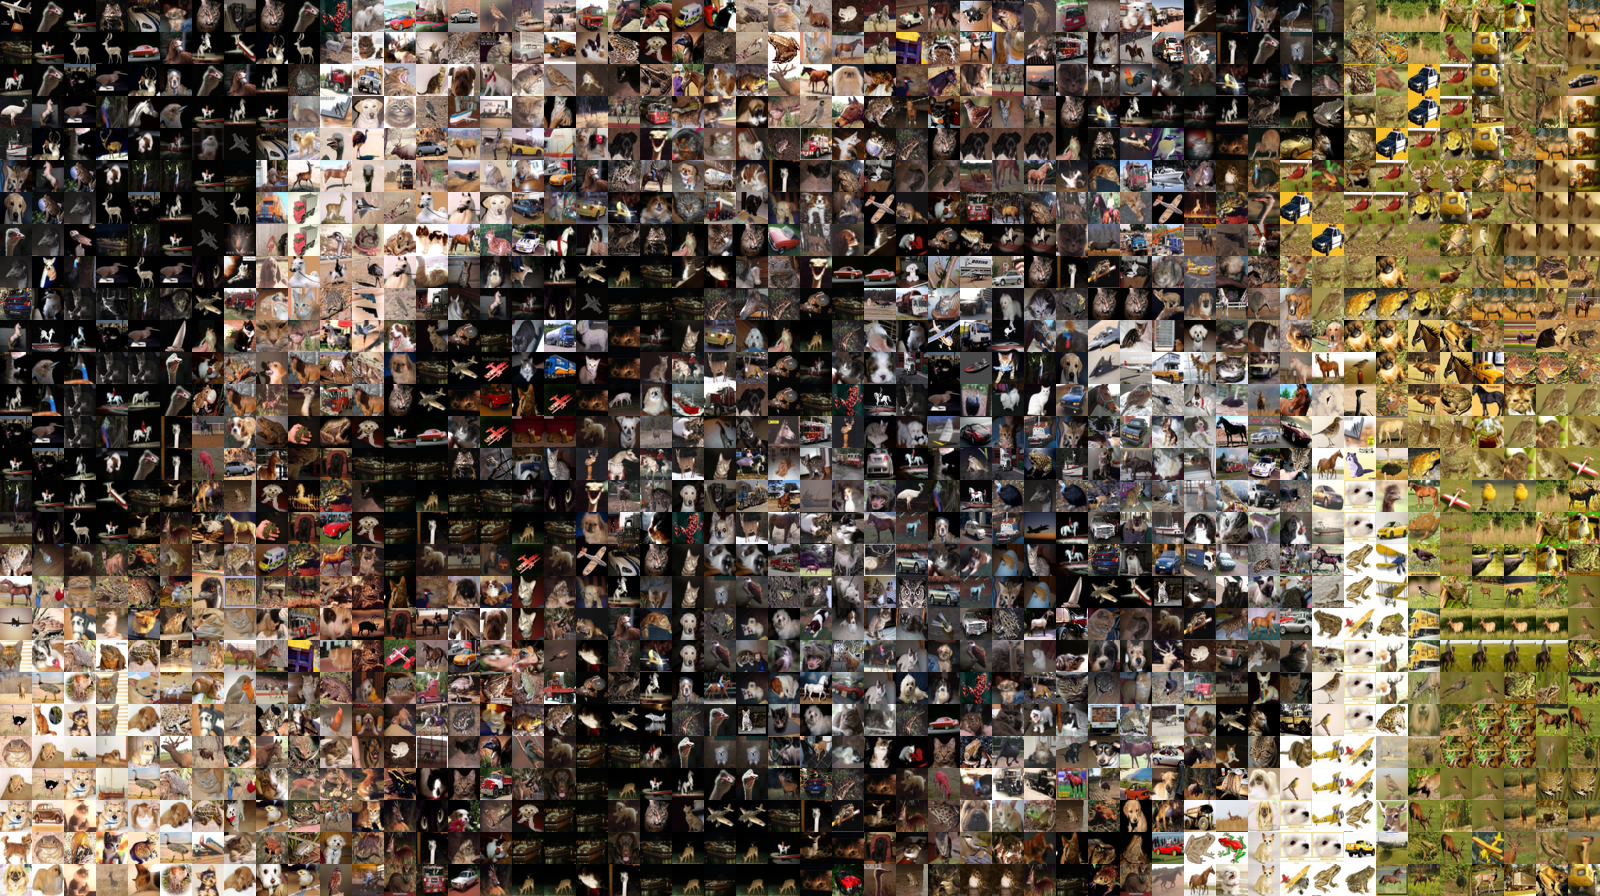
\includegraphics[width=0.45\linewidth]{mosaic-dog1-nearest}
			\caption{
				Left: Target image. 
				Right: Output of mosaicking algorithm. 
				Magnify to see patches.
			}
			\label{fig:mosaic-dog1-nearest}
		\end{figure}
		Hence, we can see that Image Mosaicking requires a somewhat abstract understanding of the image patches in order to find patches that are visually similar to the target image's patches.
		In the next section, you will learn how exactly we define similarity and why it is hard measure the ``distance'' between two images.
		
	\subsection{Metrics}
		You are probably familiar with the Euclidean distance (even if you have never heard of Euclid) and know how to measure distances on a 2D map or even in 3D space. 
		The concept of a distance or \emph{metric} (as mathematicians call it) extends to other, high-dimensional spaces.
		In general, a metric $d$ is defined by these four properties:
		\begin{align}
			d(x, y) &\geq 0 \\
			d(x, y) &= 0 \iff x = y \\
			d(x, y) &= d(y, x) \\
			d(x, z) &\leq (x, y) + d(y, z) 
		\end{align}
		These properties need to hold for all $x, y, z$.
		Don't be afraid of these formulas, they are very intuitive!
		The first inequality says that a distance is non-negative. 
		This certainly makes sense.
		The second equation simply means that the distance between two objects can only be zero if and only if the two objects are one and the same.
		This also makes sense (for example think of distances between cities in Switzerland).
		The third property says that a distance should be symmetric, that is, the distance measured from Bern to Z\"urich is the same as measured from Z\"urich to Bern.
		Finally, the third property is called the \emph{triangle inequality}. 
		It simply means that the distance is longer or equal if you take a detour, e.g.\@ 
		$d(\text{Bern, Z\"urich}) \leq d(\text{Bern, Basel}) + d(\text{Basel, Z\"urich})$.
		
		Can we define a metric on images? 
		Say we have one, then we would be able to quantitatively measure the difference between two images $A$ and $B$. 
		If $d(A, B)$ is a small number, we would say $A$ and $B$ are similar, and if the distance is large, we say they are not similar.
		But how does one compute such a number for \emph{any} pair of images (or patches in our project)?
		Is it even possible to do that?
		
	\subsection{A Simple Mosaicking Algorithm}\label{sec:simple-mosaicking}
		As an example, let's look at a naive way of comparing two patches: we compute the average color of each patch and look at the difference.
		\begin{equation}\label{eq:mean-color-distance}
			d(x, y) = \lVert \bar{x} - \bar{y} \rVert = \left\lVert \frac{1}{N} \sum_{i=1}^{N} x_i - y_i  \right\rVert
		\end{equation}
		Here, $\bar{x}$ and $\bar{y}$ denote the average/mean of patch $x$ and $y$ respectively, and $N$ is the number of pixels in each patch.
		Note that this is \emph{not} a metric. 
		Can you figure out which of the four properties of a metric are violated?
		
		Having this function $d(x, y)$ defined, we can now formulate a simple algorithm to search through the dataset and find a good patch for every patch in the target image (see algorithm~\ref{alg:nearest-neighbor}). 
		\begin{algorithm}[bt]
			\begin{algorithmic} 
				\FOR{$x$ in image}
					\STATE smallest $\leftarrow \infty$
					\STATE nearest $\leftarrow \emptyset$
					\FOR{$y$ in dataset}	
						\IF{$d(x, y) < $ smallest}
						\STATE smallest $\leftarrow d(x, y)$
						\STATE nearest $\leftarrow y$
						\ENDIF
					\ENDFOR
					\STATE replace $x$ in image with nearest
				\ENDFOR
			\end{algorithmic}
			\caption{Nearest Neighbor Search}
			\label{alg:nearest-neighbor}
		\end{algorithm}
		This algorithm is called a \emph{nearest neighbor} search. 
		It finds the patch in the dataset that is closest to the target patch (according to the distance $d(x,y)$).
		
		As explained later in the assignments, you will use nearest neighbor search and implement the average distance for your first Mosaicking algorithm in Assignment 1.
		
	\subsection{Clustering}
		Clustering in Machine Learning is used to understand structure in data. 
		It can be easily explained with a real-life example: A supermarket.
		Let's say you want to go to Migros and buy pasta, but the brand or type of pasta does not matter.
		Will you go through every shelf and look at every product individually to check if it is pasta? 
		No. 
		You probably know that there is one shelf that has all the pasta, and only pasta.
		In data science, this is called a cluster.
		A cluster is a part of the space (a shelf) that contains a certain type of data (a product category).
		Note the following important remarks about clustering.
		\begin{itemize}
			\item Every data point belongs to a cluster, and to one cluster only.
			\item Clustering only make sense if there is structure in the data (what would an ``unstructured'' supermarket look like?)
			\item Often it is unknown how many clusters there are in the data.
		\end{itemize}
		How could we use clustering for Image Mosaicking?
		The space of all images (or image patches in our case) has structure in it, and we could reason that there must be clusters for specific types of images. For example, it is reasonable to assume that it is possible to draw a boundary between daylight- and nighttime images (yielding two clusters), but it is not trivial to describe this boundary exactly.
		Another challenge is that we don't know exactly how many clusters there are or how many we \emph{need}.
		
		In the second assignment, you will get to use the \textbf{Kmeans} clustering algorithm. 
		This algorithm can find clusters in our large collection of image patches.
		It returns the following two quantities.
		\begin{itemize}
			\item A list of $N$ \emph{cluster centers}. 
			A center is an image that represents the average for the images in that cluster.
			\item A \emph{label} for each image that tells us to which cluster it belongs (a number from $1$ to $N$).
		\end{itemize}
		\begin{figure}[tb]
			\centering
			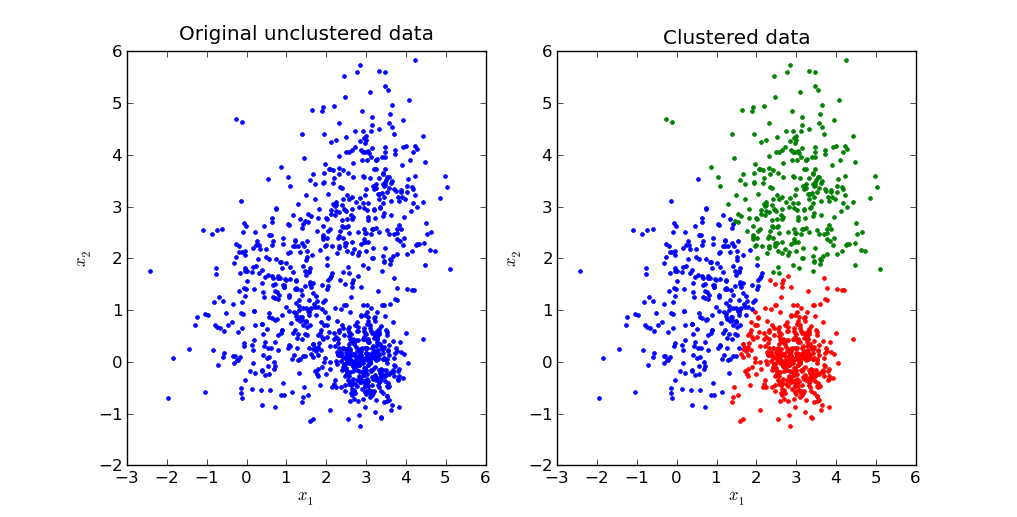
\includegraphics[width=0.8\linewidth]{clustering-example}
			\caption{
				Clustering example. 
				Left: The data before clustering. No annotations are given.
				Right: Cluster assignments after running Kmeans.
				Source: \href{https://towardsdatascience.com/k-means-data-clustering-bce3335d2203}{towardsdatascience.com}
			}
			\label{fig:clustering-example}
		\end{figure}
		In figure~\ref{fig:clustering-example} you can see an example where Kmeans was used to find three clusters in the data.
		The two axes are labeled $x_1$ and $x_2$, therefore this data lies in 2D.
		From this figure we cannot tell what the data is or what the clusters represent. 
		Can you think of two variables $x_1$ and $x_2$ that could be used for clustering?
		For example, they could be attributes for an observation made in an experiment or survey.
%		You can imagine having clusters of products in a supermarket is a good thing, because otherwise products would be mixed and scattered all over the place.

\section{Assignments}

	\subsection{Preparation}
		Take note of the following remarks before starting with the programming assignments.
		\begin{itemize}
			\item Try to understand how the code skeleton we supply is structured.
			You certainly don't have to study it in detail, because there are some technical parts that are not necessary for understanding the project.
			Start with the assignment files and see what other code is used or imported.
			
			\item If you get stuck on a problem (error message, coding, theoretical, ...) for more than 15 minutes, you should ask your tutor for help.
			
			\item Ideally, the student with the weakest programming skills should be the one coding the most, and the more experienced students should offer help and advice or do other work. 
			But feel free to discuss other options. 
			The most important thing is that everyone can contribute to the team in a meaningful way.
		\end{itemize}

	\subsection{Assignment 1a: Average Color Distance}
		\paragraph{Utility functions} 
		We will use a fixed square size of $32 \times 32$ pixels for the patches.
		Therefore, the height and width of the target image will not necessarily be divisible by 32.
		Implement the two functions \verb|number_of_patches| and \\ 
		\verb|output_image_size| in the file \verb|utils.py|.
		These helper functions are used to define the grid dimensions and to truncate the image to a size that fits the grid.
		
		\paragraph{Average feature}
		Implement the method \verb|feature| in \verb|assignment1.py|. 
		Hint: Have a look at 
		\href{https://docs.scipy.org/doc/numpy/reference/generated/numpy.mean.html}{\texttt{numpy.mean}} how to compute the average of a vector.
		Note that we are dealing with colored patches (red, green, and blue component). 
		This means that your average will be a vector of size 3, not be a scalar number.
		Ask your tutor for advice on this.
		
		\paragraph{Distance}
		Finally, implement the method \verb|distance| in \verb|assignment1.py|.
		Here you should call the \verb|feature| method to compute the features first, and then compute the difference between those features as presented in equation~\ref{eq:mean-color-distance}.
		Your method should return a single scalar number, the distance.
		
		\paragraph{Testing}
		Run the code in \verb|assignment1_test.py| to see if your computed features and distances make sense.
		You can use the generated figures in your report, poster or presentation.
		
	\subsection{Assignment 1b: Nearest Neighbor Search}
		What you have so far is a way of measuring the distance between patches.
		To find the closest match between the target patch and patches in the dataset, we will use the nearest neighbor search as discussed in section~\ref{sec:simple-mosaicking}. 
		Instead of coding it yourself, you should use an existing implementation such as the one from the Python 
		\href{http://scikit-learn.org/stable/modules/neighbors.html}{\texttt{scikit-learn}} package.
		In the \verb|get_model| method from \verb|assignment1.py| you should construct the NearestNeighbor object with two parameters:
		\begin{itemize}
			\item \verb|n_neighbor|: This is the number of closest neighbors you want to retrieve. 
			\item \verb|metric|: This is a pointer to the function that computes the distance. 
			Set it to the method you implemented.
		\end{itemize}
	
		\paragraph{Testing}
		You can test your nearest neighbor search by running \\
		\verb|assignment1_test.py|. 
		It will show you a few examples of nearest neighbors for a given patch.
		If it looks good, run the main program in \verb|assignment1.py| with your own images.
		You will notice that the program takes a long time to finish. 
		\textbf{What do you think causes the long computation time?}
		Measure the time it takes to process a single patch (directly in the code, or with a stopwatch).
	
	\subsection{Assignment 2: Clustering}
		Implement the method \verb|get_model| in the \verb|assignment2.py| file.
		This should return the initialized \verb|Kmeans| model (like \verb|NearestNeighbor| from the previous assign).
		You should provide the following arguments to Kmeans.
		\begin{itemize}
			\item \verb|n_clusters|: The number of clusters in the data. 
			You have to find a value that works best for your data. 
			Try a low number first, and then increase it.
			\item \verb|n_init|: This is the number of times the clustering is repeated with different initial cluster centers.
			\item \verb|max_iter|: The number of Kmeans iterations to be performed. 
			With each iteration, the estimated cluster centers move closer and closer to the true centers in the data.
			\item \verb|n_jobs|: The number of CPU cores that should be used for calculations. 
			This depends on your hardware. 
			Ask your tutor what value you should choose.
			\item \verb|verbose|: You should set this to \verb|True| so that you see the progress in the terminal.
		\end{itemize}
		You can find more details about the arguments for Kmeans at the link below.~\footnote{
			Documentation: \url{http://scikit-learn.org/stable/modules/generated/sklearn.cluster.KMeans.html}
		}
		Note that the clustering takes a few minutes to finish, but this needs to be done only once (for given settings).
		After it finishes, the cluster centers are saved and can be loaded every time you run the Mosaicking code in the future.
		If you would like to use the saved model, set the variable \verb|train| to \verb|False|.
		
		Once you find good settings for the clustering, test it on your own images and compare the results with nearest neighbor search.
		Also compare the runtime when using the saved model on new images.
		
	\subsection{Optional/Advanced: Features from a Neural Network}
		In this exercise you will train a neural network and apply it on the dataset to get features. 
		You will use these features in clustering instead of the raw pixel information as before.
		Neural networks are tricky! It is possible that your outputs will not look better than in the previous assignments.
		Your task is to
		\begin{itemize}
			\item train the network and compute the features for every patch in the dataset,
			\item use Kmeans clustering on the newly computed features,
			\item compare your outputs with the mosaics created in the previous assignments,
			\item conclude which of the three methods work best.
		\end{itemize}
		This exercise will require less coding and more theoretical understanding.
		Your tutor will give you an overview and tips before you start with this assignment.
	
	\subsection{Optional: Try a different dataset}
		Your tutor can show you how to use a different dataset. 
		It will require a bit of work to download and set this up.
		All your models need to be re-trained for the new dataset, therefore this is optional and should only be considered if you progress very fast.
		
		
	\subsection{Optional: Blending}
		In case your output images do not look as desired or if you want to have some more control over the end result, you can consider this blending technique.
		The idea is that you take the mosaic and superimpose the original image.
		Let $M$ be the mosaic you created and $I$ be the target image.
		You choose value $\alpha$ between zero and one and apply the formula
		\begin{equation}
			B = \alpha M + (1 - \alpha) I.
		\end{equation}
		This will create a new image $B$ which is a blend of $I$ and $M$.
		Example: $B = 0.7 \cdot M + 0.3 \cdot I$.
		If you choose $\alpha = 1$, then $B = M$, and you get back the mosaic as if you did not apply blending.
		On the other hand, $\alpha = 0$ means discard the mosaic and keep the target image, so $B = I$.

\section{Report, Poster and Presentation}

	Make sure you collect all the outputs for later use in report and presentation.
	Organize your results and give them meaningful filenames so that you remember which output corresponds to which settings you tested.
	Use a USB drive or a cloud service like Dropbox to share everything with your group members.
	You can find templates for report, poster and presentation in the download section on the SJF website.~\footnote{
	Templates: \url{https://sjf.ch/stiftung/downloads/}}
	Your tutor will communicate a review deadline for the poster and presentation and will give you feedback on those.
	

\section{Acknowledgments}
	In the name of the Institute of Computer Science and the Computer Vision Group Prof.\@ Paolo Favaro and I would like thank the foundation \emph{Schweizer Jugend forscht} for the opportunity to work with such talented young students. 
	Many thanks to the organizer Dario Moser who provided us with all necessary material, instructions and guidelines for the study week.
	Last but not least we also thank our system administrator Dr.\@ Peppo Brambilla who prepared the student computers and provided us with the necessary infrastructure.
	


\end{document}
